\documentclass{article}
\usepackage[utf8]{inputenc}
\usepackage[a4paper, total={6in, 8in}]{geometry}
\usepackage{merriweather}
\usepackage[hidelinks]{hyperref}
\usepackage{xcolor}
\usepackage{graphicx}

\title{\textbf{
CS213 - Software Systems Lab \\ 
Project Report: VaxiNO'Pandemic
}}
\author{
  B Siddharth Prabhu\\
  \href{mailto:200010003@iitdh.ac.in}{\texttt{200010003@iitdh.ac.in}}
  \and
  Ishika Sharma\\
  \href{mailto:200010020@iitdh.ac.in}{\texttt{200010020@iitdh.ac.in}}
  \and
  Nirmit Arora\\
  \href{mailto:200010034@iitdh.ac.in}{\texttt{200010034@iitdh.ac.in}}
}
\date{November 7, 2021}

\begin{document}

\maketitle

\section{Introduction and Motivation}
In these unprecedented times, we can't neglect the effects of the pandemic, and must speed up the process of vaccination. So, using our knowledge of Software Systems Lab, we decided to develop a {\color{blue}\href{https://whitelisted2.github.io/VaxiNO-Pandemic/}{portal}} to aid the drive. You can view a video overview of our project  {\color{blue}\href{https://youtu.be/0gNqwNLtwm4}{here}}.

\section{Main Tasks and Goals}
\begin{itemize}
    \item {\color{blue}\href{https://whitelisted2.github.io/VaxiNO-Pandemic/user_login_signup.html}{Login and Sign-Up}}
    \item {\color{blue}\href{https://whitelisted2.github.io/VaxiNO-Pandemic/awareness.html}{Information and Awareness}}
    \item Statistics (requires XAMPP) % using python
    \item Map of Vaccine Centres
    \item Checking Eligibility via Age
    \item Slot availability % w/ locations
    \begin{itemize}
        \item Vaccine dose type
        \item Age groups
        \item Locations
        \item If private, then fee
    \end{itemize}
    \item Certificate of Vaccination (Generation and download/ printable HTML page)
\end{itemize}
% slot availability
% html template for certificate
% map overlap
% Acknowledgements
\section{Deliverables}
\begin{itemize}
    \item HTML/CSS has been thoroughly used in the website's display features.
    \item PHP and SQL have been used to process form input, and update the database; there are multiple SQL databases.
    \item Javascript has been used to code some \texttt{onClick()} actions in the site peripherals.
    \item \LaTeX~has been used to construct and maintain this report.
    \item Python has used for statistics; it executes via \texttt{shell\_exec()} in PHP.
    \item Git and GitHub have been used for version control.
\end{itemize}

\section{Screenshots}
    \subsection{Main Page}
        \begin{figure}[hbt]
            \centering
            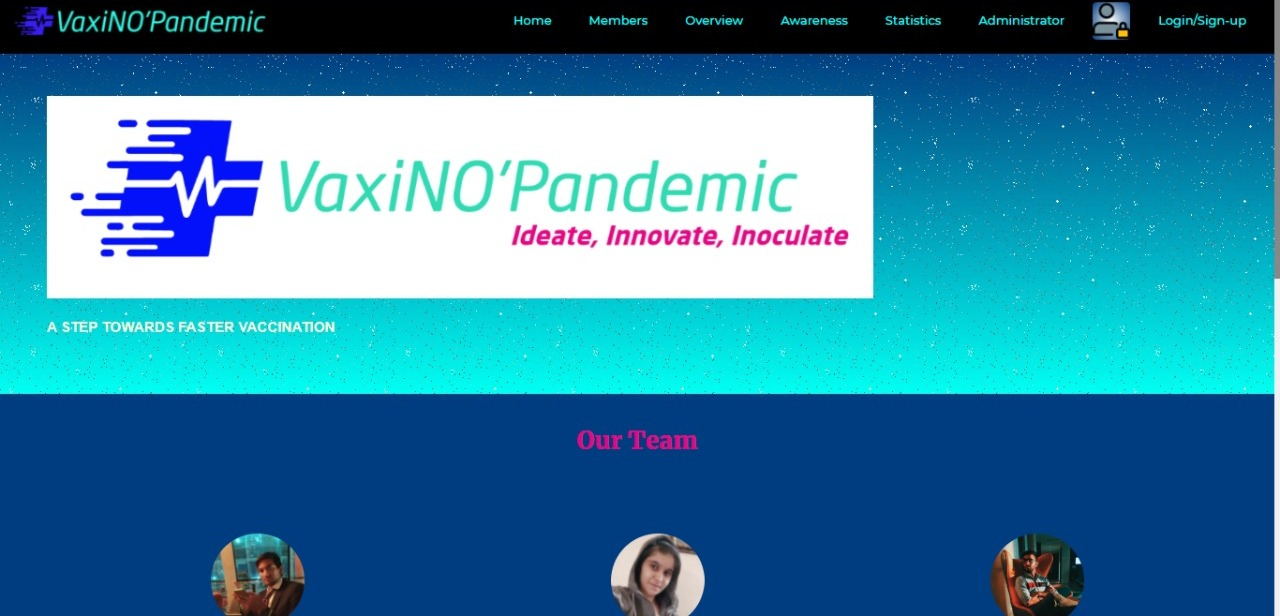
\includegraphics[scale=0.3]{mainpage.jpeg}
            \caption{Main Page}
            \label{fig:mainpage}
        \end{figure}
    \newpage
    \subsection{Embedded Map}
        \begin{figure}[hbt]
            \centering
            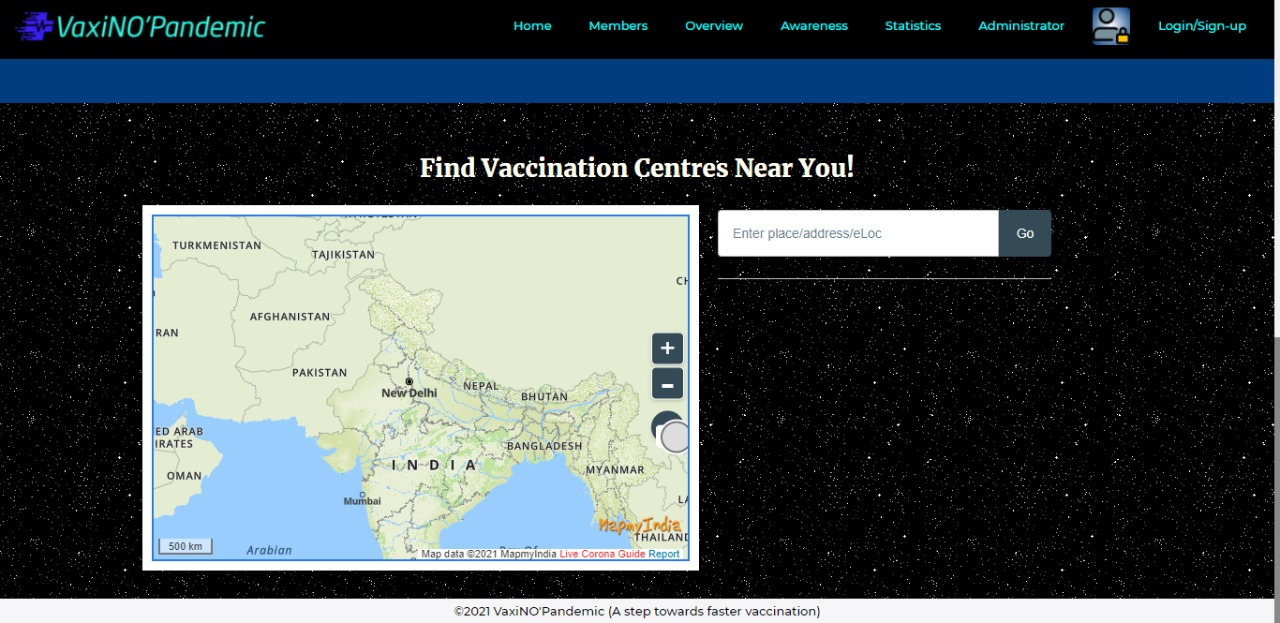
\includegraphics[scale=0.3]{maparea.jpeg}
            \caption{Map with live vaccination centers}
            \label{fig:maparea}
        \end{figure}
    \subsection{Awareness Page}
        \begin{figure}[hbt]
            \centering
            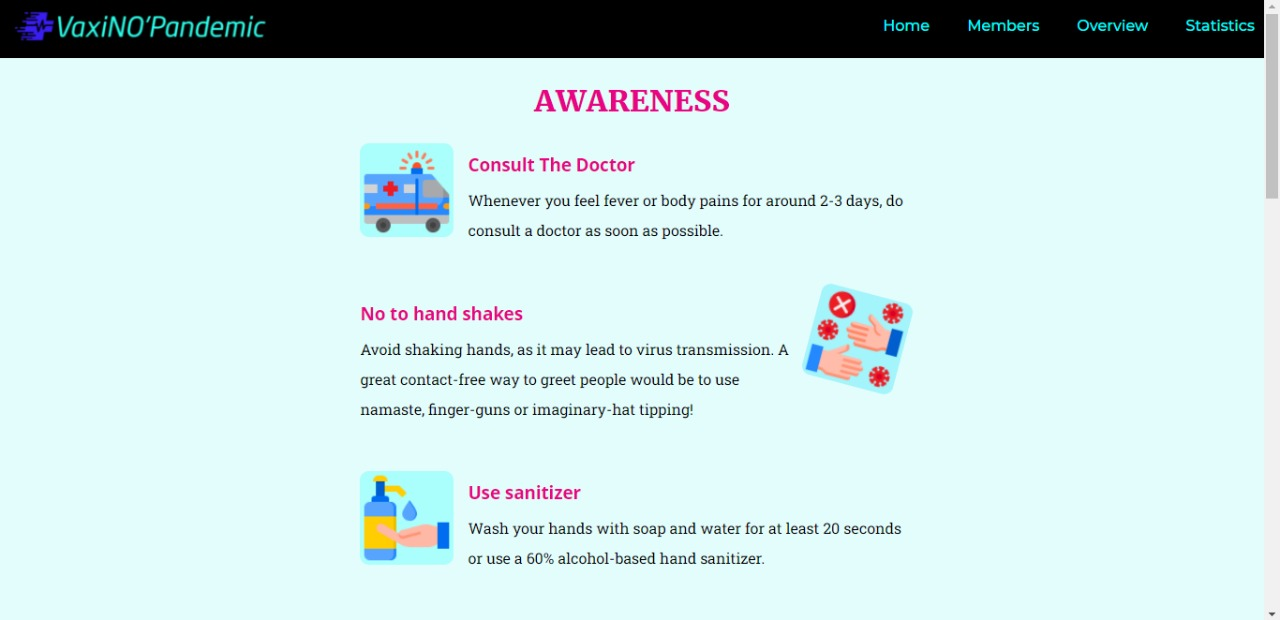
\includegraphics[scale=0.3]{awareness.jpeg}
            \caption{Awareness Page}
            \label{fig:awareness}
        \end{figure}
    \newpage
    \subsection{Statistics Page}
        \begin{figure}[hbt]
            \centering
            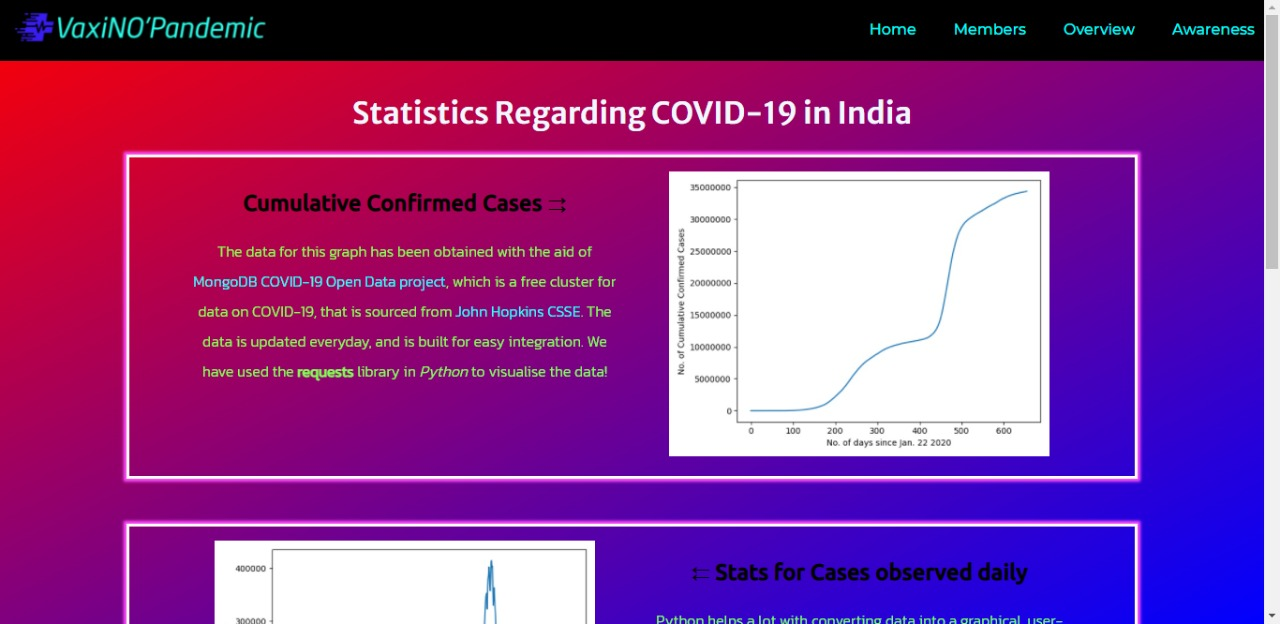
\includegraphics[scale=0.3]{stats.jpeg}
            \caption{Statistics (in the form of map) which updates daily}
            \label{fig:stats}
        \end{figure}
    \subsection{Administrator Login Page}
        \begin{figure}[hbt]
            \centering
            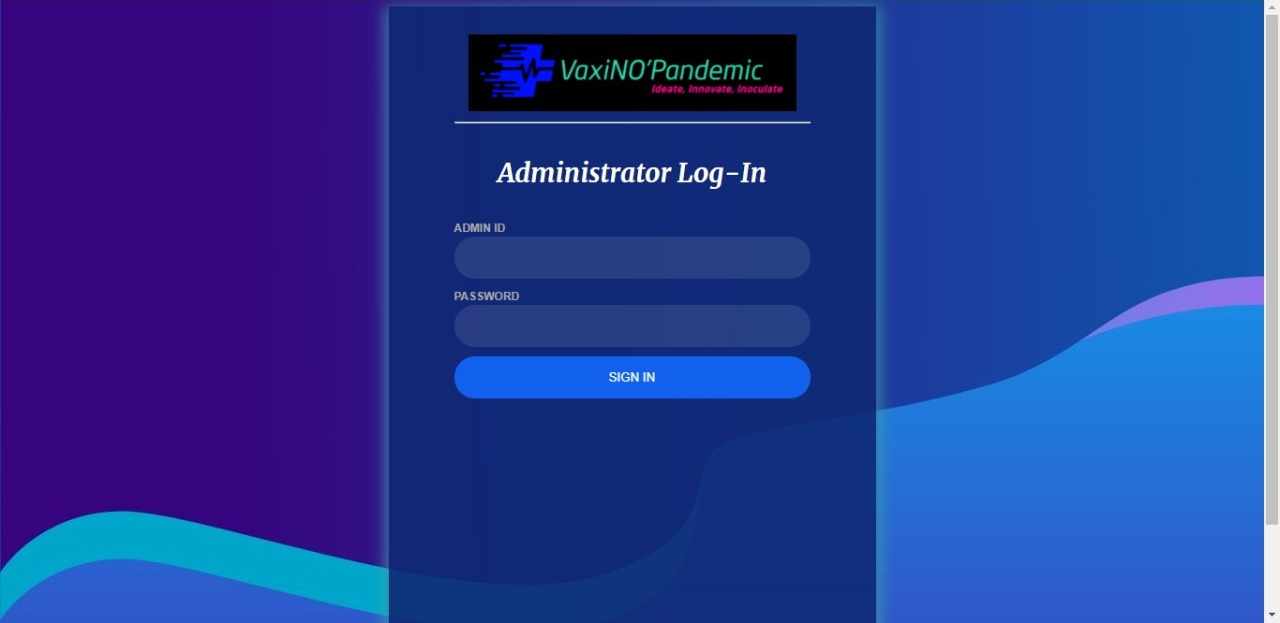
\includegraphics[scale=0.3]{adminlogin.jpeg}
            \caption{Administrator Login Page}
            \label{fig:adminlogin}
        \end{figure}
    \newpage
    \subsection{Administrator Dashboard}
        \begin{figure}[hbt]
            \centering
            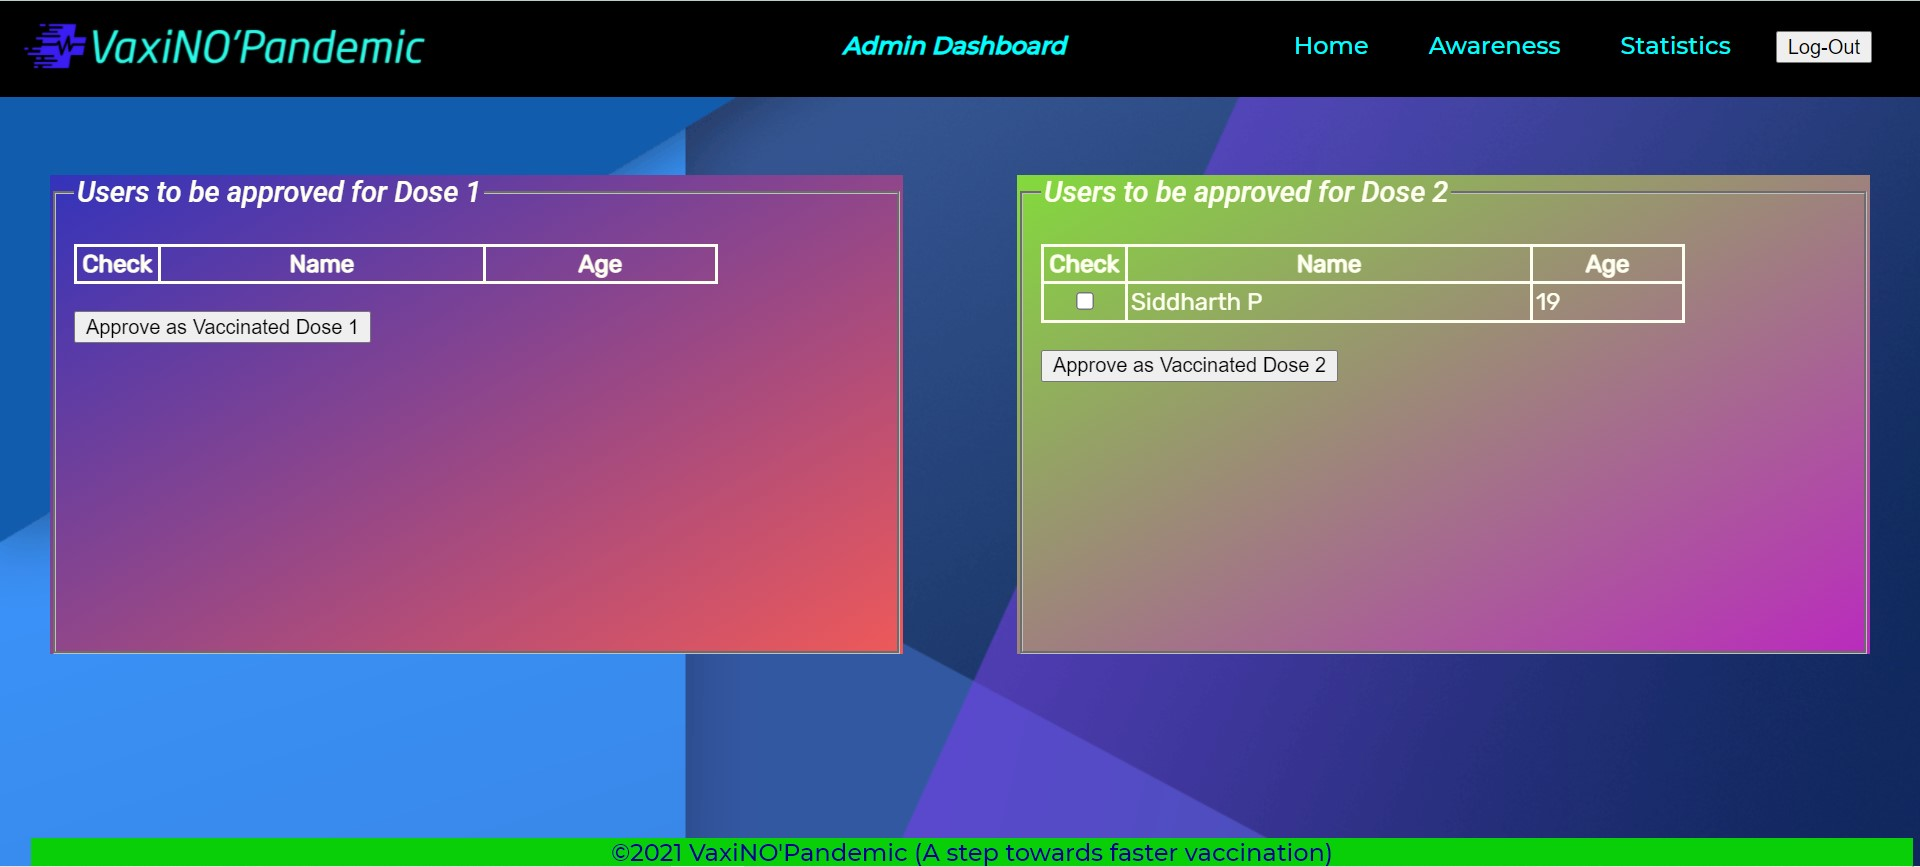
\includegraphics[scale=0.40682]{admindash.jpg}
            \caption{Administrator Dashboard}
            \label{fig:admindash}
        \end{figure}
    \subsection{User Login Page}
        \begin{figure}[hbt]
            \centering
            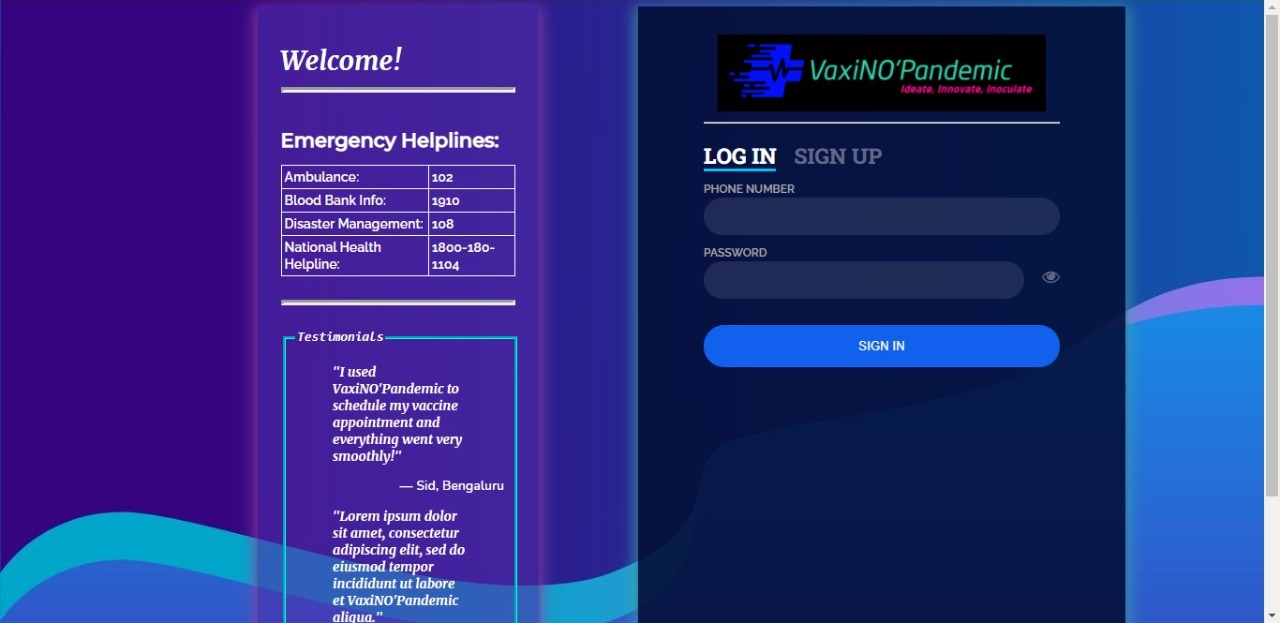
\includegraphics[scale=0.32]{userlogin.jpeg}
            \caption{User Login Page}
            \label{fig:userlogin}
        \end{figure}
    \newpage
    \subsection{User Dashboard}
        \begin{figure}[hbt]
            \centering
            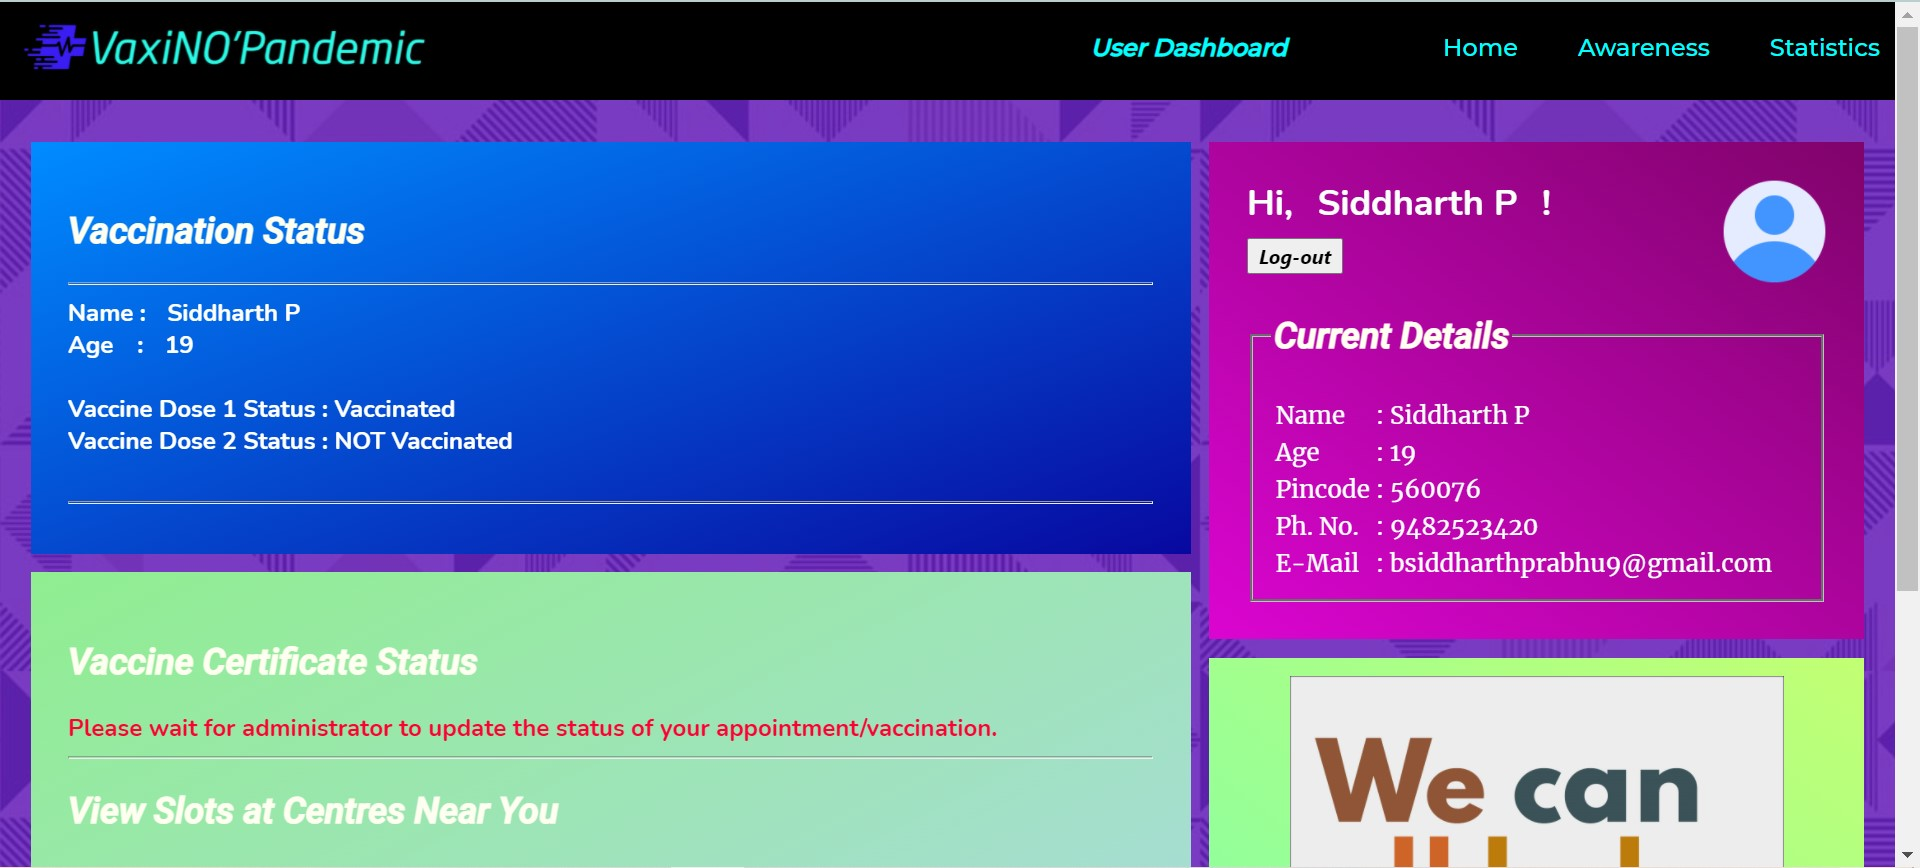
\includegraphics[scale=0.406]{userdash.jpg}
            \caption{User Dashboard}
            \label{fig:userdashboard}
        \end{figure}
    \subsection{View Slots}
        \begin{figure}[hbt]
            \centering
            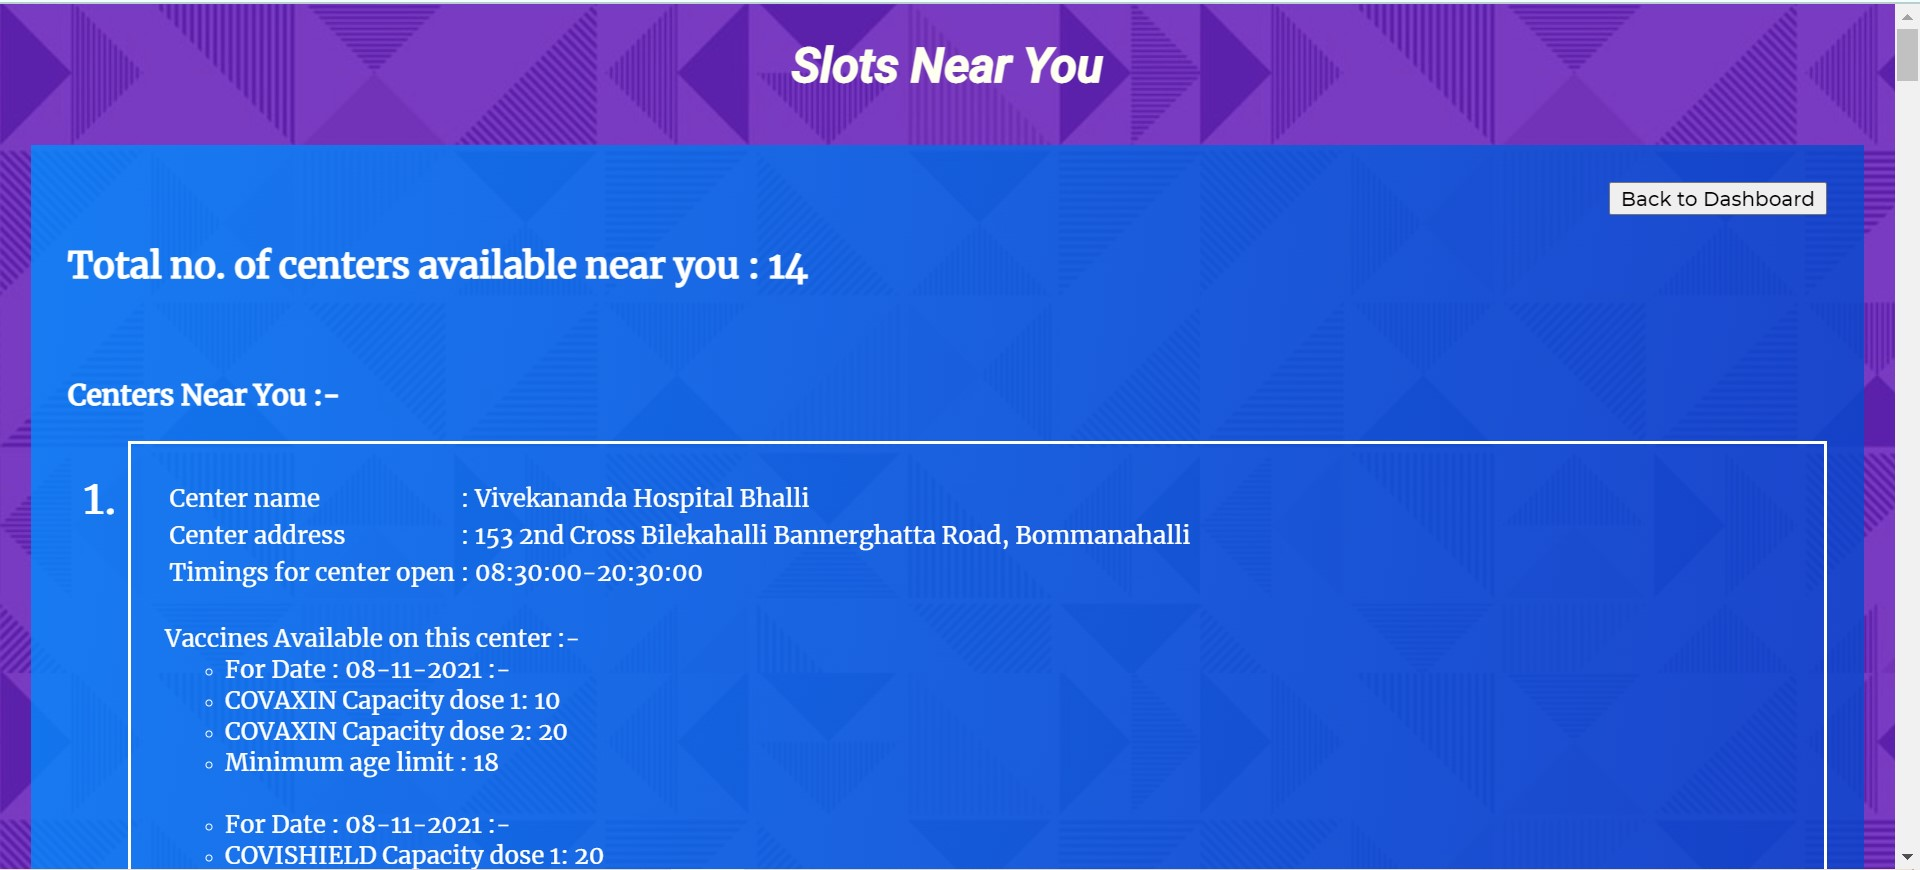
\includegraphics[scale=0.406]{slots.jpg}
            \caption{View Slots}
            \label{fig:slots}
        \end{figure}
    \newpage
    \subsection{Vaccine Certificate}
        \begin{figure}[hbt]
            \centering
            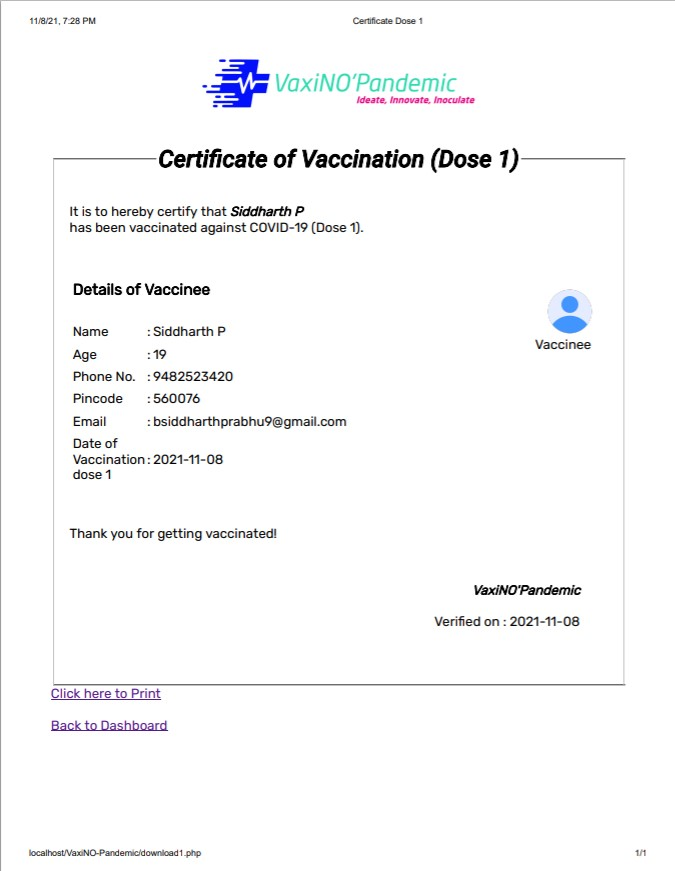
\includegraphics[scale=0.9]{cert.jpg}
            \caption{Vaccine Certificate}
            \label{fig:certificate}
        \end{figure}
    \newpage
\section{Acknowledgements}
We would like to thank the creators of the following resources, as these have been extremely valuable in the construction and maintenance this project.
\begin{description}
\item{\href{https://fonts.google.com/}{\color{blue}\textbf{Google Fonts}}} has been used profusely across the website, and has a wide variety of fonts with easy integration.
\item{\href{https://ourworldindata.org/covid-vaccinations?country=IND}{\color{blue}\textbf{Our World In Data}}} \cite{owidcoronavirus} provided us with the data related to vaccination across the country.
\item{\href{https://github.com/mongodb-developer/open-data-covid-19#collection-global}{\color{blue}\textbf{MongoDB COVID-19 Open Data project}}} gave us a data cluster that used the Johns Hopkins University (JHU) dataset. It is the backbone of the Statistics page on VaxiNO'Pandemic.
\item{\href{https://www.mapmyindia.com/api/corona/#State-wise-corona-cases}{\color{blue}\textbf{MapMyIndia}}} was our source for the "Vaccine Centres Near You" Map, and was simple to integrate into out webpage.
\item{\href{https://apisetu.gov.in/api/cowin/cowin-public-v2}{\color{blue}\textbf{API Setu}}} has been helpful in checking slots at nearby vaccine centres.
\end{description}

\bibliographystyle{IEEEtran}
\bibliography{list.bib}

\end{document}
